\section{Filer}
\subsection*{Alt er lagret i filer}
\begin{frame}{HDD}
    \begin{itemize}[<+->]
        \item Disk = permanent lagring
        \item Hard disk drive (HDD)
        \begin{itemize}
          \item Roterende magnetiske fat 
          \item Mekaniske bevegelser tar tid
        \end{itemize}
        \item Lese og skrive til disken krever:
        \begin{itemize}
          \item Posisjonere armene
          \item Vente for at riktig sektor passerer under armene
          \item Overføre data fra/til RAM
        \end{itemize}
    \end{itemize}
\end{frame}

\begin{frame}{SSD}
  \begin{itemize}[<+->]
    \item Solid State Disk (SSD)
    \begin{itemize}
      \item Ingen bevegelige deler
      \item Mye raskere enkelt lookup
      \item Erstatter hard disker i mange områder
    \end{itemize}
    \item Forskjellen på HDD og SSD
    \begin{itemize}
      \item SSD er raskt
      \item HDD er billig
    \end{itemize}
\end{itemize}
\end{frame}



\subsection*{Terminologi}
\begin{frame}{Terminologi}
  \begin{itemize}[<+->]
    \item Tabell   = File
    \item Rad      = Record
    \item Attributt = Field
  \end{itemize}
\end{frame}

\subsection*{Blocks}
\begin{frame}
  \begin{columns}
  \begin{column}{0.48\textwidth}
    \begin{figure}
        %\centering
        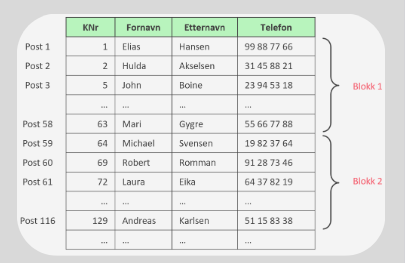
\includegraphics[height = 3.8cm]{images/blocks.png}
        \caption{En fil delt i blokker}
        \label{fig:blocks}
    \end{figure}
  \end{column}
  \begin{column}{0.48\textwidth}
    \begin{itemize}[<+->]
        \item En blokk er den minste enheten for å overføre data mellom RAM og ekstern lagring (HDD/SSD)
        \item Typisk blokk størrelse: 4KB
        \item En blokk kan generelt inneholde flere records (rader) 
    \end{itemize}
  \end{column}
  \end{columns}
\end{frame}

\subsection*{Spørretid}
\begin{frame}{Spørsmål?}
    \begin{figure}
        \centering
        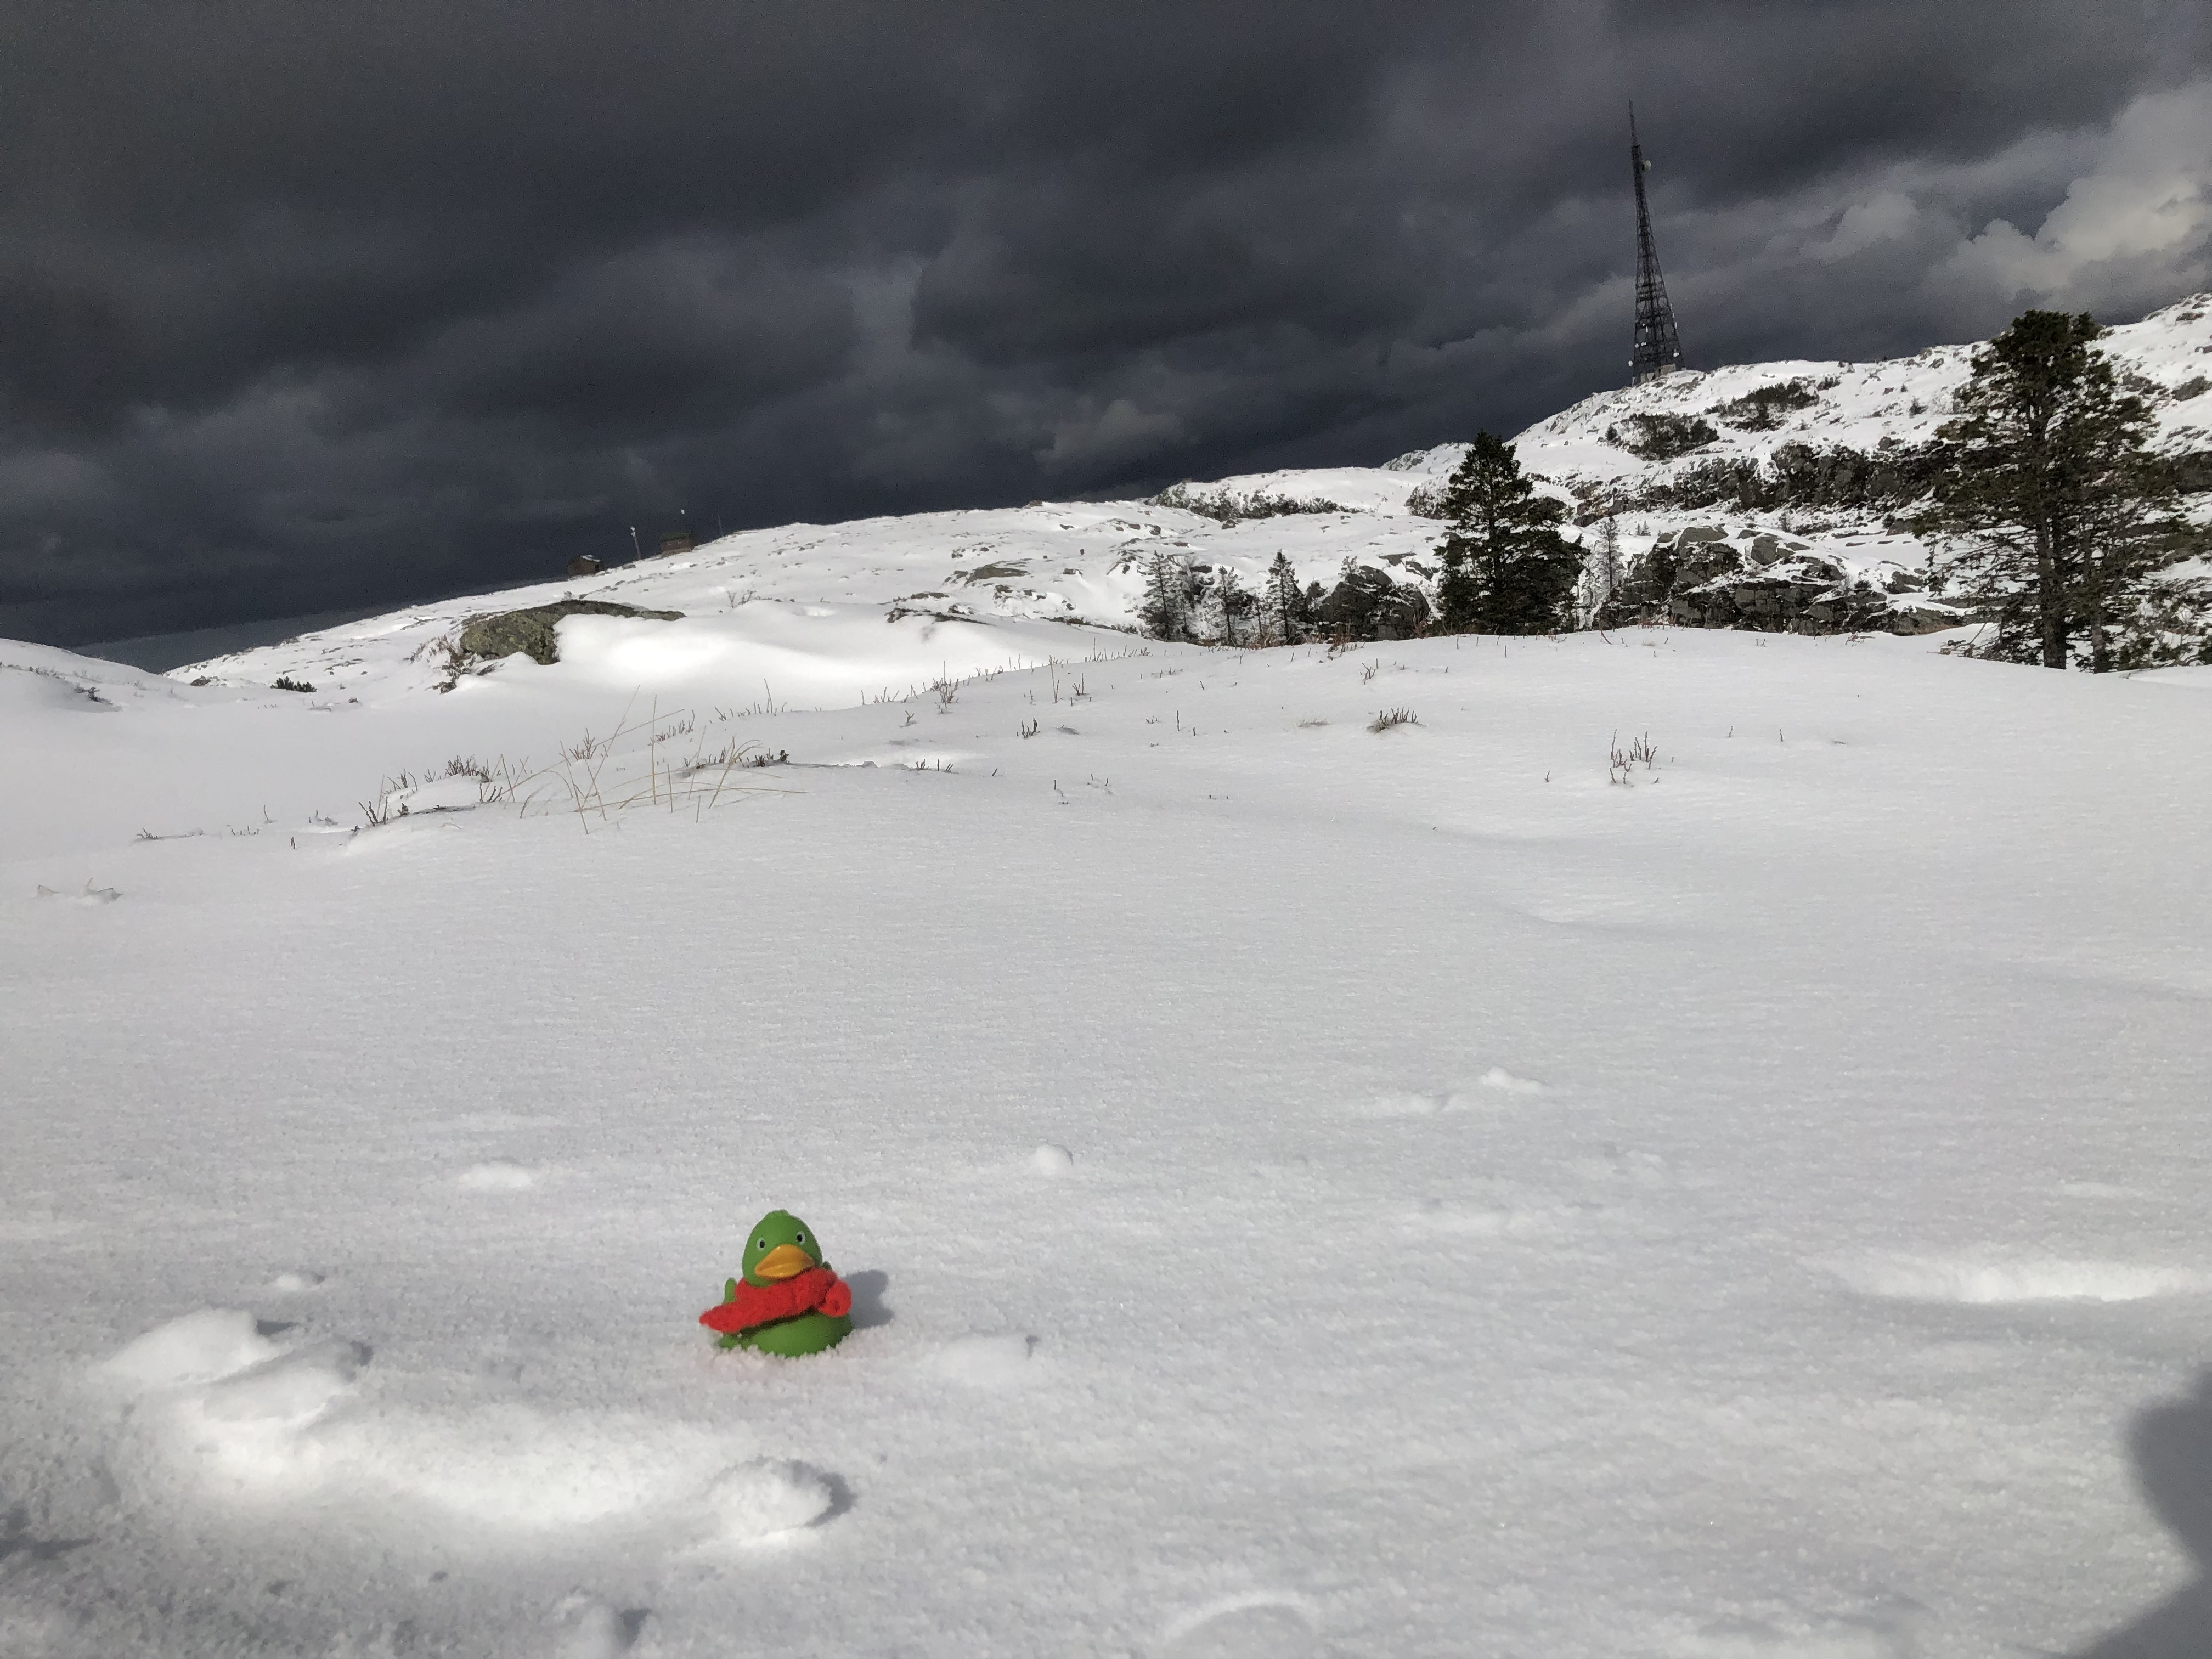
\includegraphics[height = 4.9cm]{images/guillaume7.jpg}
        \caption{Guillaume i snøen}
        \label{fig:guillaume8}
    \end{figure}
\end{frame}
